% Options for packages loaded elsewhere
\PassOptionsToPackage{unicode}{hyperref}
\PassOptionsToPackage{hyphens}{url}
\PassOptionsToPackage{dvipsnames,svgnames,x11names}{xcolor}
%
\documentclass[
  letterpaper,
  DIV=11,
  numbers=noendperiod]{scrartcl}

\usepackage{amsmath,amssymb}
\usepackage{iftex}
\ifPDFTeX
  \usepackage[T1]{fontenc}
  \usepackage[utf8]{inputenc}
  \usepackage{textcomp} % provide euro and other symbols
\else % if luatex or xetex
  \usepackage{unicode-math}
  \defaultfontfeatures{Scale=MatchLowercase}
  \defaultfontfeatures[\rmfamily]{Ligatures=TeX,Scale=1}
\fi
\usepackage{lmodern}
\ifPDFTeX\else  
    % xetex/luatex font selection
\fi
% Use upquote if available, for straight quotes in verbatim environments
\IfFileExists{upquote.sty}{\usepackage{upquote}}{}
\IfFileExists{microtype.sty}{% use microtype if available
  \usepackage[]{microtype}
  \UseMicrotypeSet[protrusion]{basicmath} % disable protrusion for tt fonts
}{}
\makeatletter
\@ifundefined{KOMAClassName}{% if non-KOMA class
  \IfFileExists{parskip.sty}{%
    \usepackage{parskip}
  }{% else
    \setlength{\parindent}{0pt}
    \setlength{\parskip}{6pt plus 2pt minus 1pt}}
}{% if KOMA class
  \KOMAoptions{parskip=half}}
\makeatother
\usepackage{xcolor}
\setlength{\emergencystretch}{3em} % prevent overfull lines
\setcounter{secnumdepth}{-\maxdimen} % remove section numbering
% Make \paragraph and \subparagraph free-standing
\makeatletter
\ifx\paragraph\undefined\else
  \let\oldparagraph\paragraph
  \renewcommand{\paragraph}{
    \@ifstar
      \xxxParagraphStar
      \xxxParagraphNoStar
  }
  \newcommand{\xxxParagraphStar}[1]{\oldparagraph*{#1}\mbox{}}
  \newcommand{\xxxParagraphNoStar}[1]{\oldparagraph{#1}\mbox{}}
\fi
\ifx\subparagraph\undefined\else
  \let\oldsubparagraph\subparagraph
  \renewcommand{\subparagraph}{
    \@ifstar
      \xxxSubParagraphStar
      \xxxSubParagraphNoStar
  }
  \newcommand{\xxxSubParagraphStar}[1]{\oldsubparagraph*{#1}\mbox{}}
  \newcommand{\xxxSubParagraphNoStar}[1]{\oldsubparagraph{#1}\mbox{}}
\fi
\makeatother


\providecommand{\tightlist}{%
  \setlength{\itemsep}{0pt}\setlength{\parskip}{0pt}}\usepackage{longtable,booktabs,array}
\usepackage{calc} % for calculating minipage widths
% Correct order of tables after \paragraph or \subparagraph
\usepackage{etoolbox}
\makeatletter
\patchcmd\longtable{\par}{\if@noskipsec\mbox{}\fi\par}{}{}
\makeatother
% Allow footnotes in longtable head/foot
\IfFileExists{footnotehyper.sty}{\usepackage{footnotehyper}}{\usepackage{footnote}}
\makesavenoteenv{longtable}
\usepackage{graphicx}
\makeatletter
\newsavebox\pandoc@box
\newcommand*\pandocbounded[1]{% scales image to fit in text height/width
  \sbox\pandoc@box{#1}%
  \Gscale@div\@tempa{\textheight}{\dimexpr\ht\pandoc@box+\dp\pandoc@box\relax}%
  \Gscale@div\@tempb{\linewidth}{\wd\pandoc@box}%
  \ifdim\@tempb\p@<\@tempa\p@\let\@tempa\@tempb\fi% select the smaller of both
  \ifdim\@tempa\p@<\p@\scalebox{\@tempa}{\usebox\pandoc@box}%
  \else\usebox{\pandoc@box}%
  \fi%
}
% Set default figure placement to htbp
\def\fps@figure{htbp}
\makeatother
% definitions for citeproc citations
\NewDocumentCommand\citeproctext{}{}
\NewDocumentCommand\citeproc{mm}{%
  \begingroup\def\citeproctext{#2}\cite{#1}\endgroup}
\makeatletter
 % allow citations to break across lines
 \let\@cite@ofmt\@firstofone
 % avoid brackets around text for \cite:
 \def\@biblabel#1{}
 \def\@cite#1#2{{#1\if@tempswa , #2\fi}}
\makeatother
\newlength{\cslhangindent}
\setlength{\cslhangindent}{1.5em}
\newlength{\csllabelwidth}
\setlength{\csllabelwidth}{3em}
\newenvironment{CSLReferences}[2] % #1 hanging-indent, #2 entry-spacing
 {\begin{list}{}{%
  \setlength{\itemindent}{0pt}
  \setlength{\leftmargin}{0pt}
  \setlength{\parsep}{0pt}
  % turn on hanging indent if param 1 is 1
  \ifodd #1
   \setlength{\leftmargin}{\cslhangindent}
   \setlength{\itemindent}{-1\cslhangindent}
  \fi
  % set entry spacing
  \setlength{\itemsep}{#2\baselineskip}}}
 {\end{list}}
\usepackage{calc}
\newcommand{\CSLBlock}[1]{\hfill\break\parbox[t]{\linewidth}{\strut\ignorespaces#1\strut}}
\newcommand{\CSLLeftMargin}[1]{\parbox[t]{\csllabelwidth}{\strut#1\strut}}
\newcommand{\CSLRightInline}[1]{\parbox[t]{\linewidth - \csllabelwidth}{\strut#1\strut}}
\newcommand{\CSLIndent}[1]{\hspace{\cslhangindent}#1}

\usepackage{booktabs}
\usepackage{longtable}
\usepackage{array}
\usepackage{multirow}
\usepackage{wrapfig}
\usepackage{float}
\usepackage{colortbl}
\usepackage{pdflscape}
\usepackage{tabu}
\usepackage{threeparttable}
\usepackage{threeparttablex}
\usepackage[normalem]{ulem}
\usepackage{makecell}
\usepackage{xcolor}
\usepackage{tabularray}
\usepackage[normalem]{ulem}
\usepackage{graphicx}
\UseTblrLibrary{booktabs}
\UseTblrLibrary{rotating}
\UseTblrLibrary{siunitx}
\NewTableCommand{\tinytableDefineColor}[3]{\definecolor{#1}{#2}{#3}}
\newcommand{\tinytableTabularrayUnderline}[1]{\underline{#1}}
\newcommand{\tinytableTabularrayStrikeout}[1]{\sout{#1}}
\KOMAoption{captions}{tableheading}
\usepackage{tikz}
\usepackage{pgfplots}
\pgfplotsset{compat=newest}
\usetikzlibrary{plotmarks}
\usetikzlibrary{arrows.meta}
\usepgfplotslibrary{patchplots}
\usepackage{grffile}
\usepackage{caption}
\usepackage[utf8]{inputenc}
\usepackage{float}
\usepackage{multirow}
\usepackage{tablefootnote}
\usepackage{pifont}
\usepackage{newunicodechar}
\usepackage{booktabs}
\usepackage{siunitx}
\usepackage{tabularx}
\newunicodechar{✓}{\ding{51}}
\usepackage{tabularray}
\floatplacement{table}{H}
\usepackage{graphicx}
\usepackage{codehigh}
\usepackage[normalem]{ulem}
\UseTblrLibrary{booktabs}
\UseTblrLibrary{siunitx}
\newcommand{\beginsupplement}{ \setcounter{table}{0} \renewcommand{\thetable}{A\arabic{table}} \setcounter{figure}{0} \renewcommand{\thefigure}{A\arabic{figure}}}
\makeatletter
\@ifpackageloaded{caption}{}{\usepackage{caption}}
\AtBeginDocument{%
\ifdefined\contentsname
  \renewcommand*\contentsname{Table of contents}
\else
  \newcommand\contentsname{Table of contents}
\fi
\ifdefined\listfigurename
  \renewcommand*\listfigurename{List of Figures}
\else
  \newcommand\listfigurename{List of Figures}
\fi
\ifdefined\listtablename
  \renewcommand*\listtablename{List of Tables}
\else
  \newcommand\listtablename{List of Tables}
\fi
\ifdefined\figurename
  \renewcommand*\figurename{Figure}
\else
  \newcommand\figurename{Figure}
\fi
\ifdefined\tablename
  \renewcommand*\tablename{Table}
\else
  \newcommand\tablename{Table}
\fi
}
\@ifpackageloaded{float}{}{\usepackage{float}}
\floatstyle{ruled}
\@ifundefined{c@chapter}{\newfloat{codelisting}{h}{lop}}{\newfloat{codelisting}{h}{lop}[chapter]}
\floatname{codelisting}{Listing}
\newcommand*\listoflistings{\listof{codelisting}{List of Listings}}
\makeatother
\makeatletter
\makeatother
\makeatletter
\@ifpackageloaded{caption}{}{\usepackage{caption}}
\@ifpackageloaded{subcaption}{}{\usepackage{subcaption}}
\makeatother

\usepackage{bookmark}

\IfFileExists{xurl.sty}{\usepackage{xurl}}{} % add URL line breaks if available
\urlstyle{same} % disable monospaced font for URLs
\hypersetup{
  pdftitle={Supplemental Material for Complementarity in Alliances: How strategic compatibility and hierarchy promote efficient cooperation in international security},
  pdfauthor={J Andrés Gannon},
  colorlinks=true,
  linkcolor={blue},
  filecolor={Maroon},
  citecolor={Blue},
  urlcolor={Blue},
  pdfcreator={LaTeX via pandoc}}


\title{Supplemental Material for \emph{Complementarity in Alliances: How
strategic compatibility and hierarchy promote efficient cooperation in
international security}}
\author{J Andrés Gannon}
\date{}

\begin{document}
\maketitle


\beginsupplement

\tableofcontents

\newpage

\section{A. Descriptive statistics}\label{a.-descriptive-statistics}

\begin{table}

\caption{\label{tbl-summstats}Summary statistics of model variables.
Year polynomials omitted from table.}

\centering{

\centering
\resizebox{\ifdim\width>\linewidth 1\linewidth\else\width\fi}{!}{
\begin{tblr}[         %% tabularray outer open
]                     %% tabularray outer close
{                     %% tabularray inner open
colspec={Q[]Q[]Q[]Q[]Q[]Q[]Q[]Q[]},
column{1}={halign=l,},
column{2}={halign=l,},
column{3}={halign=l,},
column{4}={halign=l,},
column{5}={halign=l,},
column{6}={halign=l,},
column{7}={halign=l,},
column{8}={halign=l,},
}                     %% tabularray inner close
\toprule
& Unique & Missing Pct. & Mean & SD & Min & Median & Max \\ \midrule %% TinyTableHeader
Year & 45 & 0 & 1991.27 & 12.99 & 1970.00 & 1990.00 & 2014.00 \\
Division of labor & 2131 & 4 & 0.33 & 0.26 & 0.00 & 0.29 & 1.00 \\
Strategic compatibility & 815 & 0 & 0.34 & 0.27 & 0.00 & 0.29 & 1.00 \\
Hierarchy & 645 & 0 & 0.23 & 0.24 & 0.00 & 0.15 & 1.00 \\
Peacetime coordination & 4 & 4 & 0.84 & 0.84 & 0.00 & 1.00 & 2.00 \\
Democracy ratio & 70 & 2 & 0.39 & 0.41 & 0.00 & 0.30 & 1.00 \\
Proportion contiguous & 60 & 0 & 0.37 & 0.44 & 0.00 & 0.12 & 1.00 \\
Maximum distance (log) & 87 & 0 & 5.76 & 3.92 & 0.00 & 7.66 & 9.85 \\
Number of rivals (log) & 38 & 0 & 2.06 & 0.73 & 0.00 & 2.20 & 3.61 \\
Alliance members (log) & 31 & 0 & 1.17 & 0.83 & 0.69 & 0.69 & 3.50 \\
Alliance age (avg) & 335 & 0 & 19.41 & 14.68 & 0.00 & 16.00 & 64.24 \\
\bottomrule
\end{tblr}
}

}

\end{table}%

Most of the missing data comes from the division of labor variable and
is primarily due to two alliances for which there are many missing
values -- ATOP ID 3830 (bilateral defense pact between France and
Comoros signed in 1978) is missing 37 values and ATOP ID 3900 (treaty
establishing the Organization of Eastern Caribbean States between
Antigua, Dominica, Grenada, Montserrat, St.~Kitts/Nevis, Saint Lucia,
and St.~Vincent and the Grenadines) is missing 34.

\newpage

\section{B. Manuscript model supplementary
info}\label{b.-manuscript-model-supplementary-info}

\subsection{Ordered beta results
table}\label{ordered-beta-results-table}

\begin{table}

\caption{\label{tbl-obr}Log odds coefficient estimates. Time
dependencies modeled as year cubic splines given computational
constraints for year fixed effects.}

\centering{

\centering
\begin{tblr}[         %% tabularray outer open
]                     %% tabularray outer close
{                     %% tabularray inner open
colspec={Q[]Q[]},
column{1}={halign=l,},
column{2}={halign=c,},
hline{20}={1,2}{solid, 0.05em, black},
}                     %% tabularray inner close
\toprule
& (1) \\ \midrule %% TinyTableHeader
Strategic Compatibility & 2.020          \\
& [1.613, 2.531] \\
Hierarchy               & 4.407          \\
& [3.060, 6.446] \\
Peacetime Coordination  & 1.108          \\
& [1.045, 1.176] \\
Democracy Ratio         & 1.586          \\
& [1.359, 1.839] \\
Contiguity Ratio        & 1.161          \\
& [0.775, 1.743] \\
Maximum Distance (log)  & 0.985          \\
& [0.937, 1.036] \\
Number of Rivals (log)  & 1.410          \\
& [1.286, 1.553] \\
Number of Members (log) & 0.809          \\
& [0.749, 0.870] \\
Alliance Age (avg)      & 0.996          \\
& [0.991, 1.000] \\
Num.Obs.                & 2280           \\
RMSE                    & 0.22           \\
\bottomrule
\end{tblr}

}

\end{table}%

\newpage

\section{C. Alternate explanatory
variables}\label{c.-alternate-explanatory-variables}

\subsection{Strategic Compatibility}\label{strategic-compatibility}

I define strategic compatibility as ``consistency of states' security
interests and agreement on the nature of the international threat
environment''. To provide more detail, including exact definitions from
the original data sources, state B is considered a part of state A's
threat environment if it meets any of the following conditions:

\begin{enumerate}
\def\labelenumi{\arabic{enumi})}
\item
  Strategic rivalry - states A and B have an un-directed strategic
  rivalry if they ``regard each other as (a) competitors, (b) the source
  of actual or latent threats that pose some possibility of becoming
  militarized, and (c) enemies'' (Thompson 2001, 560). The data comes
  from Thompson, Sakuwa, and Suhas (2021, 34--46) and codings are used
  without modification.
\item
  Peace scale rivalry - states A and B have an un-directed peace scale
  relationship coded as ``severe rivalry'', meaning ``the states see one
  another as enemies and competitors\ldots which encourage rivals to
  handle their contested issues via frequent and intense uses of
  violence.'' or states A and B are non-allied and have an un-directed
  peace scale relationship coded as ``lesser rivalry'', meaning that
  ``The sentiments of threat, enmity and competition that remain---along
  with the persistence of unresolved issues---mean that lesser rivalries
  still experience isolated violent episodes (e.g.~militarized disputes
  or MIDs), diplomatic hostility, and non-violent crises'' (Diehl,
  Goertz, and Gallegos 2021, 610). I use version 3.1.
\item
  Politically relevant threat environment - state B is contiguous or a
  great power \emph{and} it is non-allied with a kappa chance-corrected
  alliance similarity score below the population median. Contiguity and
  great power status are a commonly used scope condition for politically
  relevant dyads (Maoz 1996, 168) and the decision to subset that to
  dyads with inconsistent foreign policy orientations comes from Leeds
  and Savun (2007). The modifications I make relative to Leeds and Savun
  (2007) concern expanding the definition of contiguous to include less
  than 25 miles of water (M. A. Benson 2005; Bennett 2006; Braumoeller
  and Carson 2011) and instead of using the population's median s-score
  as a threshold for similar foreign policy orientation, I use the kappa
  chance-corrected measure to minimize statistical bias in s-score
  comparisons (Cohen 1960; Häge 2011; Chiba, Johnson, and Leeds 2015).
\end{enumerate}

There are 1,358,924 directed-dyad years from 1970 to 2014 of which
40,428 categorize state B as being a member of state A's threat
environment. Figure~\ref{fig-strcompcompare} shows the overlap among the
3 criteria used to determine each state's threat environment.

\begin{figure}

\centering{

\pandocbounded{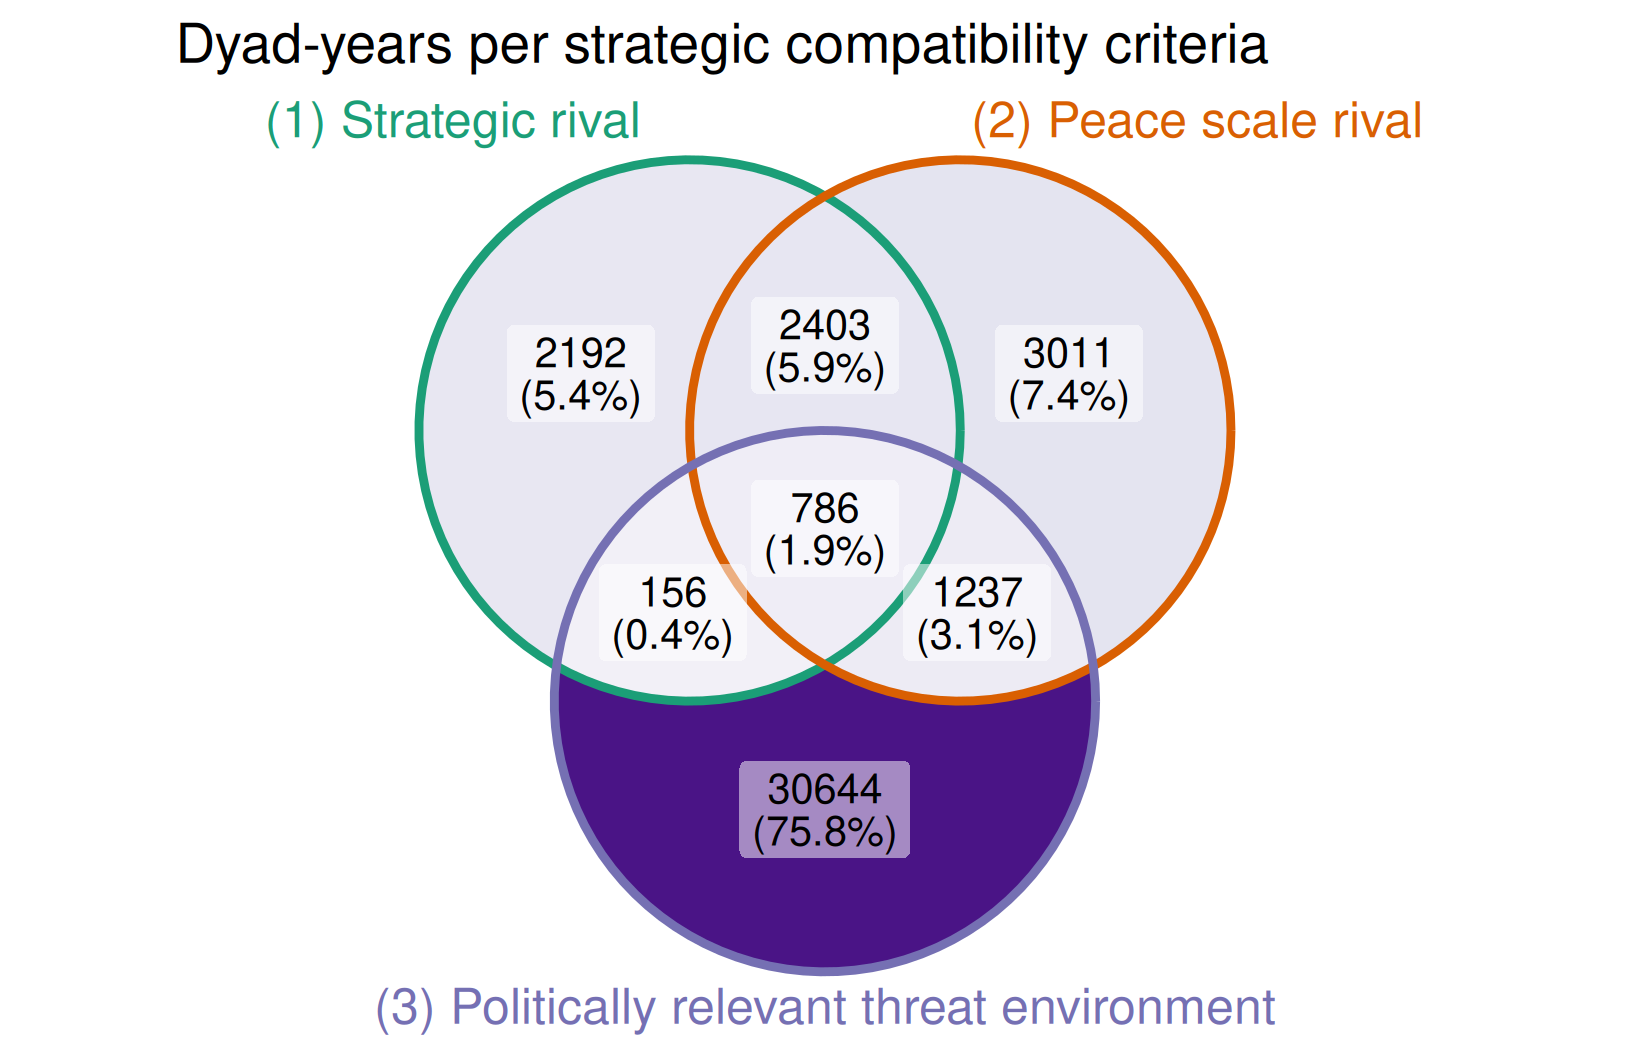
\includegraphics[keepaspectratio]{DoDL_Appendix_files/figure-pdf/fig-strcompcompare-1.png}}

}

\caption{\label{fig-strcompcompare}Overlap among strategic compatibility
criteria. Counts refer to number of dyad-years.}

\end{figure}%

Criteria 1 is most similar to Poast (2019, 52--57) and Criteria 3 is
most similar to Leeds and Savun (2007, 1127) with the following
modifications:

\begin{itemize}
\item
  Poast (2019) uses a count of states as threats, while I weight each
  threat by their CINC score. If all NATO states view Russia as a threat
  and only the US views Cuba as a threat, the relative military salience
  of Russia and Cuba should be considered.
\item
  Poast (2019, 93) addresses the absence of asymmetric rivalries in
  Thompson (2001) by adding contiguous great powers as a strategic
  rival. I address that through Criteria 3 in my measure.
\item
  Poast (2019) makes strategic compatibility binary with high (low)
  strategic compatibility being above (below) the sample median, I keep
  it continuous and scale it by the highest observed value in the full
  population.
\item
  Poast (2019) combines strategic compatibility (what I measure) with
  operational compatibility which addresses agreement about how to use
  military force against a threat based on offensive or defense war time
  doctrine (Bennett and Stam 1996; Stam 1996; Reiter and Stam 1998). I
  do not include a measure of operational compatibility given its
  similarity to the dependent variable, lack of vary within alliances,
  and absence of data for my time period.
\item
  Leeds and Savun (2007) use un-weighted ATOP s-score, but I use the
  kappa-corrected s-score measure as suggested by (Häge 2011; Cohen
  1960).
\item
  Leeds and Savun (2007) exclude all alliance partners from a state's
  threat environment. Since allies do sometimes have serious rivalries
  and conflicts (Greece-Turkey in NATO, India-Pakistan in SCO,
  Russia-Georgia, Russia-Ukraine, Armenia-Azerbaijan in CIS, etc) I
  allow an ally to be in your threat environment if it is coded as a
  strategic rivalry or a peace level ``serious rivalry'' (Weitsman 1997;
  Bearce, Flanagan, and Floros 2006).
\end{itemize}

I find consistent results using weighted and un-weighted s-scores
measuring alliance portfolio similarity using ATOP which has previously
been used to measure variation in strength of alliance ties (Gibler and
Rider 2004; Chiba, Johnson, and Leeds 2015; Fordham and Poast 2016). I
opt against using UN voting similarity as a measure of strategic
compatibility because of recognized problems with chance agreement (Häge
2011) the high frequency of consensus decisions (Häge and Hug 2016), and
agenda effects bias year-over-year change (Bailey, Strezhnev, and Voeten
2017).

\begin{table}

\caption{\label{tbl-altstrcomp}Coefficient estimates with alternate
variables for strategic compatibility.}

\centering{

\centering
\resizebox{\ifdim\width>\linewidth 1\linewidth\else\width\fi}{!}{
\begin{talltblr}[         %% tabularray outer open
entry=none,label=none,
note{}={* p < 0.05, ** p < 0.01, *** p < 0.001},
note{ }={All models include alliance-clustered standard errors.},
]                     %% tabularray outer close
{                     %% tabularray inner open
colspec={Q[]Q[]Q[]},
column{1}={halign=l,},
column{2}={halign=c,},
column{3}={halign=c,},
hline{18}={1,2,3}{solid, 0.05em, black},
}                     %% tabularray inner close
\toprule
& (1) & (2) \\ \midrule %% TinyTableHeader
S-score (weighted)      & 0.320** &         \\
& (0.099) &         \\
S-score (unweighted)    &         & 0.422*  \\
&         & (0.193) \\
Hierarchy               & 0.367** & 0.372** \\
& (0.113) & (0.124) \\
Democracy Ratio         & 0.093   & 0.106*  \\
& (0.048) & (0.053) \\
Contiguity Ratio        & 0.101   & 0.213   \\
& (0.113) & (0.130) \\
Maximum Distance (log)  & 0.009   & 0.026   \\
& (0.014) & (0.017) \\
Number of Members (log) & -0.045  & -0.050  \\
& (0.024) & (0.029) \\
Alliance Age (avg)      & 0.002   & 0.001   \\
& (0.001) & (0.002) \\
Num.Obs.                & 2381    & 2381    \\
R2                      & 0.211   & 0.197   \\
R2 Adj.                 & 0.207   & 0.194   \\
AIC                     & -240.3  & -199.9  \\
BIC                     & -176.8  & -136.3  \\
RMSE                    & 0.23    & 0.23    \\
\bottomrule
\end{talltblr}
}

}

\end{table}%

\newpage

\subsection{Hierarchy}\label{hierarchy}

Alliance power asymmetry has been measured using a variety of similar
measures. While none are identical to the new measure of hierarchy
created, one would still expect the coefficient sign to be consistent.
These measures are defined in the original texts as follows:

\begin{itemize}
\item
  potential military capacity (B. V. Benson and Clinton 2016, 873--75):
  log of the summed CINC score of all alliance members, presence of a
  major power, mean geographic distance between all alliance pairs, log
  of the number of alliance members, mean s-score of all pairs of
  alliance members, and the average Polity IV score of all alliance
  members.
\item
  alliance depth (B. V. Benson and Clinton 2016, 872--73): ``military
  contact, common defense policy, integrated command, military aid,
  military basing, specific contribution, organization, economic aid,
  and secret.''
\item
  peacetime coordination (Leeds and Anac 2005, 188--91): ordinal
  variable coded \emph{high} if alliances have an integrated military
  command during peacetime and wartime, have a common defense policy
  obligation, and have joint troop placement agreements. Coded
  \emph{moderate} if peacetime official military contact is required,
  there is a formal military organization for coordination, one party is
  required to provide training or technology to another, and there are
  specific plans to subordinate one military to another during conflict.
  Coded \emph{low} otherwise.
\item
  latent alliance depth (Alley 2021, 932): ordinal factor analysis
  measuring ``additional policy coordination and military cooperation
  beyond a promise of military support. Defense cooperation in a deep
  alliance can take many forms, including an integrated military
  command, military aid, common defense policies, basing rights,
  international organizations, specific contribution requirements or
  companion military agreements.''
\item
  CINC dispersion (Gibler and Rider 2004, 316): ``captures the dispersal
  of capabilities in an alliance; it ranges from 0 (when the
  capabilities in the alliance are equally distributed) to 1 (when one
  state holds all of the capabilities in the alliance). In this formula,
  \(\sqrt{\sum_{i=1}^{n}(Si)^2-\frac{1}{n}/(1-\frac{1}{n})}\), \(Si\)
  denotes \(i\)'s share of the alliance's total capabilities, and \(n\)
  is the number of allies in the alliance.''
\item
  CINC asymmetry (B. V. Benson and Clinton 2016, 888): ``measured by
  subtracting the CINC scores of the strongest and weakest pair of
  alliance members.''
\item
  great power participation (Gibler and Rider 2004; Leeds and Savun
  2007, 188): Ratio variable indicating how many alliance members are
  great powers.
\end{itemize}

\begin{table}

\caption{\label{tbl-althierarchy}Coefficient estimates with alternate
variables for hierarchy.}

\centering{

\centering
\resizebox{\ifdim\width>\linewidth 1\linewidth\else\width\fi}{!}{
\begin{talltblr}[         %% tabularray outer open
entry=none,label=none,
note{}={* p < 0.05, ** p < 0.01, *** p < 0.001},
note{ }={All models include alliance-clustered standard errors.},
]                     %% tabularray outer close
{                     %% tabularray inner open
colspec={Q[]Q[]Q[]Q[]Q[]Q[]Q[]Q[]},
column{1}={halign=l,},
column{2}={halign=c,},
column{3}={halign=c,},
column{4}={halign=c,},
column{5}={halign=c,},
column{6}={halign=c,},
column{7}={halign=c,},
column{8}={halign=c,},
hline{30}={1,2,3,4,5,6,7,8}{solid, 0.05em, black},
}                     %% tabularray inner close
\toprule
& (1) & (2) & (3) & (4) & (5) & (6) & (7) \\ \midrule %% TinyTableHeader
Strategic Compatibility     & 0.243*** & 0.066    & 0.062    & 0.054    & 0.130*   & 0.114*  & 0.151*** \\
& (0.059)  & (0.046)  & (0.044)  & (0.045)  & (0.051)  & (0.044) & (0.040)  \\
Potential Military Capacity & 0.095*** &          &          &          &          &         &          \\
& (0.020)  &          &          &          &          &         &          \\
Alliance Depth              &          & 0.059*** &          &          &          &         &          \\
&          & (0.012)  &          &          &          &         &          \\
Peacetime Coord             &          &          & 0.049**  &          &          &         &          \\
&          &          & (0.018)  &          &          &         &          \\
Latent Depth                &          &          &          & 0.032    &          &         &          \\
&          &          &          & (0.020)  &          &         &          \\
CINC Dispersal              &          &          &          &          & 0.081**  &         &          \\
&          &          &          &          & (0.028)  &         &          \\
CINC Asymmetry              &          &          &          &          &          & 0.574*  &          \\
&          &          &          &          &          & (0.286) &          \\
Great power ratio           &          &          &          &          &          &         & 0.260**  \\
&          &          &          &          &          &         & (0.088)  \\
Democracy Ratio             & 0.118**  & 0.159*** & 0.173*** & 0.136**  & 0.162*** & 0.141** & 0.122**  \\
& (0.044)  & (0.044)  & (0.039)  & (0.045)  & (0.045)  & (0.043) & (0.043)  \\
Contiguity Ratio            & -0.167   & -0.154   & -0.193   & -0.139   & -0.041   & -0.086  & -0.095   \\
& (0.112)  & (0.120)  & (0.112)  & (0.122)  & (0.121)  & (0.115) & (0.113)  \\
Maximum Distance (log)      & -0.023   & -0.027   & -0.030*  & -0.020   & -0.007   & -0.011  & -0.015   \\
& (0.015)  & (0.016)  & (0.015)  & (0.016)  & (0.017)  & (0.016) & (0.016)  \\
Number of Rivals (log)      & 0.030    & 0.097*** & 0.092*** & 0.092*** & 0.060*   & 0.063*  & 0.042    \\
& (0.031)  & (0.022)  & (0.022)  & (0.023)  & (0.027)  & (0.025) & (0.028)  \\
Number of Members (log)     & 0.000    & -0.010   & -0.005   & -0.022   & -0.049   & -0.012  & 0.033    \\
& (0.018)  & (0.019)  & (0.015)  & (0.020)  & (0.026)  & (0.020) & (0.028)  \\
Alliance Age (avg)          & 0.000    & 0.003*   & 0.002    & 0.002    & 0.001    & 0.000   & 0.001    \\
& (0.002)  & (0.001)  & (0.001)  & (0.001)  & (0.001)  & (0.001) & (0.001)  \\
Num.Obs.                    & 2007     & 2007     & 2280     & 2339     & 2379     & 2379    & 2379     \\
R2                          & 0.279    & 0.280    & 0.263    & 0.222    & 0.239    & 0.227   & 0.244    \\
R2 Adj.                     & 0.275    & 0.276    & 0.260    & 0.218    & 0.235    & 0.224   & 0.240    \\
AIC                         & -326.6   & -330.5   & -417.7   & -251.9   & -324.3   & -288.2  & -339.7   \\
BIC                         & -259.4   & -263.2   & -348.9   & -182.8   & -255.0   & -218.9  & -270.5   \\
RMSE                        & 0.22     & 0.22     & 0.22     & 0.23     & 0.22     & 0.23    & 0.22     \\
\bottomrule
\end{talltblr}
}

}

\end{table}%

\newpage

\subsection{Interaction term}\label{interaction-term}

\begin{table}

\caption{\label{tbl-interaction}Coefficient estimates with interaction
term.}

\centering{

\centering
\resizebox{\ifdim\width>\linewidth 1\linewidth\else\width\fi}{!}{
\begin{talltblr}[         %% tabularray outer open
entry=none,label=none,
note{}={* p < 0.05, ** p < 0.01, *** p < 0.001},
note{ }={All models include alliance clustered standard errors.},
]                     %% tabularray outer close
{                     %% tabularray inner open
colspec={Q[]Q[]Q[]Q[]Q[]Q[]Q[]},
cell{1}{2}={c=2,}{halign=c,},
cell{1}{4}={c=2,}{halign=c,},
cell{1}{6}={c=2,}{halign=c,},
column{1}={halign=l,},
column{2}={halign=c,},
column{3}={halign=c,},
column{4}={halign=c,},
column{5}={halign=c,},
column{6}={halign=c,},
column{7}={halign=c,},
hline{21}={1,2,3,4,5,6,7}{solid, 0.05em, black},
}                     %% tabularray inner close
\toprule
& Year Polynomials &  & Year FE &  & Multilevel Model &  \\ \cmidrule[lr]{2-3}\cmidrule[lr]{4-5}\cmidrule[lr]{6-7}
& (1) & (2) & (3) & (4) & (5) & (6) \\ \midrule %% TinyTableHeader
Strategic Compatibility & 0.219*** & 0.183*  & 0.220*** & 0.191*  & 0.221*** & 0.189***  \\
& (0.051)  & (0.090) & (0.053)  & (0.092) & (0.023)  & (0.030)   \\
Hierarchy               & 0.479*** & 0.385*  & 0.462*** & 0.372*  & 0.452*** & 0.373***  \\
& (0.072)  & (0.167) & (0.073)  & (0.170) & (0.037)  & (0.057)   \\
Strat Comp*Hierarchy    & -0.239   & -0.155  & -0.205   & -0.139  & -0.175   & -0.110    \\
& (0.198)  & (0.200) & (0.197)  & (0.203) & (0.096)  & (0.099)   \\
Democracy Ratio         &          & 0.116*  &          & 0.115*  &          & 0.115***  \\
&          & (0.046) &          & (0.047) &          & (0.017)   \\
Contiguity Ratio        &          & -0.131  &          & -0.144  &          & -0.146**  \\
&          & (0.106) &          & (0.105) &          & (0.045)   \\
Maximum Distance (log)  &          & -0.025  &          & -0.027  &          & -0.026*** \\
&          & (0.015) &          & (0.015) &          & (0.006)   \\
Number of Rivals (log)  &          & 0.061*  &          & 0.057   &          & 0.064***  \\
&          & (0.029) &          & (0.029) &          & (0.010)   \\
Number of Members (log) &          & -0.029  &          & -0.028  &          & -0.032*** \\
&          & (0.019) &          & (0.019) &          & (0.008)   \\
Alliance Age (avg)      &          & 0.000   &          & 0.000   &          & 0.000     \\
&          & (0.001) &          & (0.001) &          & (0.000)   \\
Num.Obs.                & 2398     & 2280    & 2398     & 2280    & 2398     & 2280      \\
R2                      & 0.208    & 0.285   & 0.234    & 0.307   &          &           \\
R2 Adj.                 & 0.206    & 0.281   & 0.219    & 0.290   &          &           \\
AIC                     & -230.6   & -482.7  & -228.8   & -472.2  & -156.8   & -338.4    \\
BIC                     & -190.1   & -402.4  & 48.7     & -156.9  & -122.2   & -263.9    \\
RMSE                    & 0.23     & 0.22    & 0.23     & 0.21    & 0.23     & 0.21      \\
\bottomrule
\end{talltblr}
}

}

\end{table}%

\newpage

\section{D. Alternate and additional
controls}\label{d.-alternate-and-additional-controls}

\subsection{Alternate controls for
democracy}\label{alternate-controls-for-democracy}

The models in the manuscript operationalize democracy as the proportion
of alliance members that have a Polity score greater than 6. The results
are robust to other operationalizations of regime type commonly used in
the literature like average Polity score (B. V. Benson and Clinton
2016), lowest Polity score based on the ``weakest link'' principle
(Oneal and Russett 1997; Fordham and Poast 2016), largest difference in
Polity scores (Gibler and Rider 2004; Fordham and Poast 2016), and
whether all members are of the same regime type. To address missingness
in Polity data, I also includes controls using the Marquez (2016)
extension of the UDS latent variable measure (Pemstein, Meserve, and
Melton 2017).

\begin{table}

\caption{\label{tbl-altdemo}Coefficient estimates with alternate
democracy variables.}

\centering{

\centering
\resizebox{\ifdim\width>\linewidth 1\linewidth\else\width\fi}{!}{
\begin{talltblr}[         %% tabularray outer open
entry=none,label=none,
note{}={* p < 0.05, ** p < 0.01, *** p < 0.001},
note{ }={All models include alliance-clustered standard errors.},
]                     %% tabularray outer close
{                     %% tabularray inner open
colspec={Q[]Q[]Q[]Q[]Q[]Q[]Q[]Q[]},
column{1}={halign=l,},
column{2}={halign=c,},
column{3}={halign=c,},
column{4}={halign=c,},
column{5}={halign=c,},
column{6}={halign=c,},
column{7}={halign=c,},
column{8}={halign=c,},
hline{32}={1,2,3,4,5,6,7,8}{solid, 0.05em, black},
}                     %% tabularray inner close
\toprule
& (1) & (2) & (3) & (4) & (5) & (6) & (7) \\ \midrule %% TinyTableHeader
Strategic Compatibility & 0.163** & 0.160*   & 0.178**  & 0.166*   & 0.164** & 0.158*   & 0.180**  \\
& (0.059) & (0.063)  & (0.062)  & (0.064)  & (0.057) & (0.064)  & (0.058)  \\
Hierarchy               & 0.308*  & 0.397*** & 0.433*** & 0.421*** & 0.333** & 0.413*** & 0.396*** \\
& (0.120) & (0.109)  & (0.111)  & (0.113)  & (0.123) & (0.114)  & (0.107)  \\
Polity (avg)            & 0.008** &          &          &          &         &          &          \\
& (0.003) &          &          &          &         &          &          \\
Polity (lowest)         &         & 0.003    &          &          &         &          &          \\
&         & (0.002)  &          &          &         &          &          \\
Polity (difference)     &         &          & 0.005    &          &         &          &          \\
&         &          & (0.003)  &          &         &          &          \\
Same regime type        &         &          &          & -0.045   &         &          &          \\
&         &          &          & (0.032)  &         &          &          \\
UDS (avg)               &         &          &          &          & 0.067*  &          &          \\
&         &          &          &          & (0.026) &          &          \\
UDS (lowest)            &         &          &          &          &         & 0.025    &          \\
&         &          &          &          &         & (0.019)  &          \\
UDS (difference)        &         &          &          &          &         &          & 0.088**  \\
&         &          &          &          &         &          & (0.029)  \\
Peacetime Coordination  & 0.038*  & 0.040*   & 0.034*   & 0.036*   & 0.034*  & 0.038*   & 0.028    \\
& (0.017) & (0.017)  & (0.016)  & (0.016)  & (0.016) & (0.017)  & (0.016)  \\
Contiguity Ratio        & -0.145  & -0.091   & -0.086   & -0.069   & -0.070  & -0.037   & -0.030   \\
& (0.109) & (0.103)  & (0.109)  & (0.107)  & (0.117) & (0.107)  & (0.099)  \\
Maximum Distance (log)  & -0.027  & -0.019   & -0.018   & -0.016   & -0.019  & -0.013   & -0.012   \\
& (0.015) & (0.014)  & (0.015)  & (0.015)  & (0.015) & (0.014)  & (0.014)  \\
Number of Rivals (log)  & 0.065*  & 0.058*   & 0.038    & 0.045    & 0.067*  & 0.057*   & 0.033    \\
& (0.027) & (0.027)  & (0.024)  & (0.024)  & (0.028) & (0.028)  & (0.023)  \\
Number of Members (log) & -0.027  & -0.030   & -0.037   & -0.034   & -0.041  & -0.037   & -0.063** \\
& (0.020) & (0.019)  & (0.020)  & (0.021)  & (0.021) & (0.020)  & (0.020)  \\
Alliance Age (avg)      & 0.000   & 0.000    & 0.001    & 0.001    & 0.000   & 0.000    & 0.001    \\
& (0.001) & (0.001)  & (0.002)  & (0.001)  & (0.001) & (0.001)  & (0.001)  \\
Num.Obs.                & 2280    & 2280     & 2280     & 2280     & 2299    & 2299     & 2299     \\
R2                      & 0.288   & 0.273    & 0.278    & 0.274    & 0.295   & 0.277    & 0.307    \\
R2 Adj.                 & 0.284   & 0.269    & 0.274    & 0.270    & 0.291   & 0.273    & 0.303    \\
AIC                     & -493.7  & -445.5   & -462.1   & -449.2   & -510.6  & -454.0   & -550.8   \\
BIC                     & -419.2  & -371.0   & -387.6   & -374.7   & -436.0  & -379.4   & -476.2   \\
RMSE                    & 0.22    & 0.22     & 0.22     & 0.22     & 0.22    & 0.22     & 0.21     \\
\bottomrule
\end{talltblr}
}

}

\end{table}%

\newpage

\subsection{Alternate controls for
geography}\label{alternate-controls-for-geography}

Instead of the maximum alliance-dyad distance, Bak (2018) measures the
logged mean capital-to-capital distance between all alliance-dyads,
treating contiguous states as distance = 0. Model (1) uses Bak (2018)'
distance measure exclusively and Model (2) uses it as a replacement for
maximum distance.

\begin{table}

\caption{\label{tbl-altgeog}Coefficient estimates with alternate
geography variables.}

\centering{

\centering
\resizebox{\ifdim\width>\linewidth 1\linewidth\else\width\fi}{!}{
\begin{talltblr}[         %% tabularray outer open
entry=none,label=none,
note{}={* p < 0.05, ** p < 0.01, *** p < 0.001},
note{ }={All models include alliance-clustered standard errors.},
]                     %% tabularray outer close
{                     %% tabularray inner open
colspec={Q[]Q[]Q[]},
column{1}={halign=l,},
column{2}={halign=c,},
column{3}={halign=c,},
hline{20}={1,2,3}{solid, 0.05em, black},
}                     %% tabularray inner close
\toprule
& (1) & (2) \\ \midrule %% TinyTableHeader
Strategic Compatibility & 0.154*  & 0.155*  \\
& (0.062) & (0.061) \\
Hierarchy               & 0.344** & 0.333** \\
& (0.116) & (0.117) \\
Peacetime Coordination  & 0.035*  & 0.038*  \\
& (0.017) & (0.017) \\
Democracy Ratio         & 0.108*  & 0.115*  \\
& (0.044) & (0.045) \\
Contiguity Ratio        &         & -0.130  \\
&         & (0.119) \\
Mean Distance (log)     & -0.009  & -0.025  \\
& (0.005) & (0.016) \\
Number of Rivals (log)  & 0.056*  & 0.063*  \\
& (0.025) & (0.027) \\
Number of Members (log) & -0.044* & -0.042* \\
& (0.017) & (0.017) \\
Alliance Age (avg)      & 0.000   & 0.000   \\
& (0.001) & (0.001) \\
Num.Obs.                & 2280    & 2280    \\
R2                      & 0.281   & 0.283   \\
R2 Adj.                 & 0.278   & 0.279   \\
AIC                     & -474.0  & -478.7  \\
BIC                     & -405.2  & -404.2  \\
RMSE                    & 0.22    & 0.22    \\
\bottomrule
\end{talltblr}
}

}

\end{table}%

\subsection{Additional controls for NATO, US, and Cold
War}\label{additional-controls-for-nato-us-and-cold-war}

\begin{table}

\caption{\label{tbl-morectrls}Coefficient estimates with additional
control variables.}

\centering{

\centering
\resizebox{\ifdim\width>\linewidth 1\linewidth\else\width\fi}{!}{
\begin{talltblr}[         %% tabularray outer open
entry=none,label=none,
note{}={* p < 0.05, ** p < 0.01, *** p < 0.001},
note{ }={All models include alliance-clustered standard errors.},
]                     %% tabularray outer close
{                     %% tabularray inner open
colspec={Q[]Q[]Q[]Q[]},
column{1}={halign=l,},
column{2}={halign=c,},
column{3}={halign=c,},
column{4}={halign=c,},
hline{26}={1,2,3,4}{solid, 0.05em, black},
}                     %% tabularray inner close
\toprule
& (1) & (2) & (3) \\ \midrule %% TinyTableHeader
Strategic Compatibility & 0.140*  & 0.166**  & 0.161*  \\
& (0.066) & (0.059)  & (0.062) \\
Hierarchy               & 0.311*  & 0.426*** & 0.323** \\
& (0.121) & (0.114)  & (0.119) \\
Peacetime Coordination  & 0.042*  & 0.029    & 0.039*  \\
& (0.018) & (0.016)  & (0.017) \\
Democracy Ratio         & 0.121*  & 0.140**  & 0.113*  \\
& (0.046) & (0.050)  & (0.046) \\
Contiguity Ratio        & -0.128  & -0.089   & -0.133  \\
& (0.107) & (0.111)  & (0.105) \\
Maximum Distance (log)  & -0.025  & -0.018   & -0.025  \\
& (0.015) & (0.015)  & (0.014) \\
Number of Rivals (log)  & 0.066*  & 0.074**  & 0.064*  \\
& (0.027) & (0.026)  & (0.027) \\
Number of Members (log) & -0.022  & -0.046*  & -0.029  \\
& (0.021) & (0.019)  & (0.019) \\
Alliance Age (avg)      & 0.000   & 0.000    & 0.000   \\
& (0.001) & (0.001)  & (0.001) \\
NATO/Warsaw Pact        & -0.055  &          &         \\
& (0.042) &          &         \\
United States member    &         & -0.096*  &         \\
&         & (0.046)  &         \\
Cold War                &         &          & -0.070* \\
&         &          & (0.032) \\
Num.Obs.                & 2280    & 2280     & 2280    \\
R2                      & 0.286   & 0.292    & 0.287   \\
R2 Adj.                 & 0.282   & 0.288    & 0.283   \\
AIC                     & -485.1  & -505.3   & -488.6  \\
BIC                     & -404.9  & -425.1   & -408.3  \\
RMSE                    & 0.22    & 0.22     & 0.22    \\
\bottomrule
\end{talltblr}
}

}

\end{table}%

\newpage

\section{E. Other model
specifications}\label{e.-other-model-specifications}

\subsection{Panel-corrected standard
errors}\label{panel-corrected-standard-errors}

\begin{table}

\caption{\label{tbl-pcse}Coefficient estimates using panel-corrected
standard errors.}

\centering{

\centering
\resizebox{\ifdim\width>\linewidth 1\linewidth\else\width\fi}{!}{
\begin{talltblr}[         %% tabularray outer open
entry=none,label=none,
note{}={* p < 0.05, ** p < 0.01, *** p < 0.001},
note{ }={All models cluster standard errors by alliance and year.},
]                     %% tabularray outer close
{                     %% tabularray inner open
colspec={Q[]Q[]Q[]Q[]Q[]},
cell{1}{2}={c=2,}{halign=c,},
cell{1}{4}={c=2,}{halign=c,},
column{1}={halign=l,},
column{2}={halign=c,},
column{3}={halign=c,},
column{4}={halign=c,},
column{5}={halign=c,},
hline{21}={1,2,3,4,5}{solid, 0.05em, black},
}                     %% tabularray inner close
\toprule
& Year Polynomials &  & Year Fixed Effects &  \\ \cmidrule[lr]{2-3}\cmidrule[lr]{4-5}
& (1) & (2) & (3) & (4) \\ \midrule %% TinyTableHeader
Strategic Compatibility & 0.186*** & 0.153*  & 0.192*** & 0.165*  \\
& (0.049)  & (0.065) & (0.050)  & (0.066) \\
Hierarchy               & 0.403*** & 0.320*  & 0.397*** & 0.313*  \\
& (0.073)  & (0.122) & (0.072)  & (0.123) \\
Peacetime Coordination  &          & 0.039*  &          & 0.039*  \\
&          & (0.017) &          & (0.017) \\
Democracy Ratio         &          & 0.118*  &          & 0.116*  \\
&          & (0.046) &          & (0.047) \\
Contiguity Ratio        &          & -0.127  &          & -0.140  \\
&          & (0.117) &          & (0.117) \\
Maximum Distance (log)  &          & -0.025  &          & -0.026  \\
&          & (0.016) &          & (0.016) \\
Number of Rivals (log)  &          & 0.064*  &          & 0.060*  \\
&          & (0.028) &          & (0.028) \\
Number of Members (log) &          & -0.029  &          & -0.027  \\
&          & (0.023) &          & (0.023) \\
Alliance Age (avg)      &          & 0.000   &          & 0.000   \\
&          & (0.001) &          & (0.001) \\
Num.Obs.                & 2398     & 2280    & 2398     & 2280    \\
R2                      & 0.206    & 0.284   & 0.232    & 0.307   \\
R2 Adj.                 & 0.204    & 0.281   & 0.217    & 0.290   \\
AIC                     & -226.4   & -482.2  & -226.2   & -472.2  \\
BIC                     & -191.8   & -407.7  & 45.5     & -162.7  \\
RMSE                    & 0.23     & 0.22    & 0.23     & 0.21    \\
\bottomrule
\end{talltblr}
}

}

\end{table}%

\newpage

\subsection{Bayesian multi-level
model}\label{bayesian-multi-level-model}

A Bayesian multi-level model produces posterior distributions for the
expected division of labor conditional on strategic compatibility and
hierarchy (Bürkner 2017). Since alliances may differ in both the
baseline expectation for the dependent variable as well as how they
change over time, a Bayesian multi-level model accounts for
alliance-level heterogeneity by allowing a random intercept and slope
for each alliance nested within each year (Shor et al. 2007). As a
result, alliance-specific deviations from the population average caused
by things like alliance design or treaty depth are accounted for.

Figure~\ref{fig-bayesmlm} shows the results of the model run on 4 MCMC
chains with 4,000 iterations per chain. The marginal trend is calculated
for each independent variable conditional on the random effects of each
alliance. In these results, strategic compatibility has a strong
positive association with division of labor where the model results
suggest greater than a 95\% probability that the true marginal effect is
greater than 0. The same is true for hierarchy.

\begin{figure}

\begin{minipage}{0.50\linewidth}

\centering{

\pandocbounded{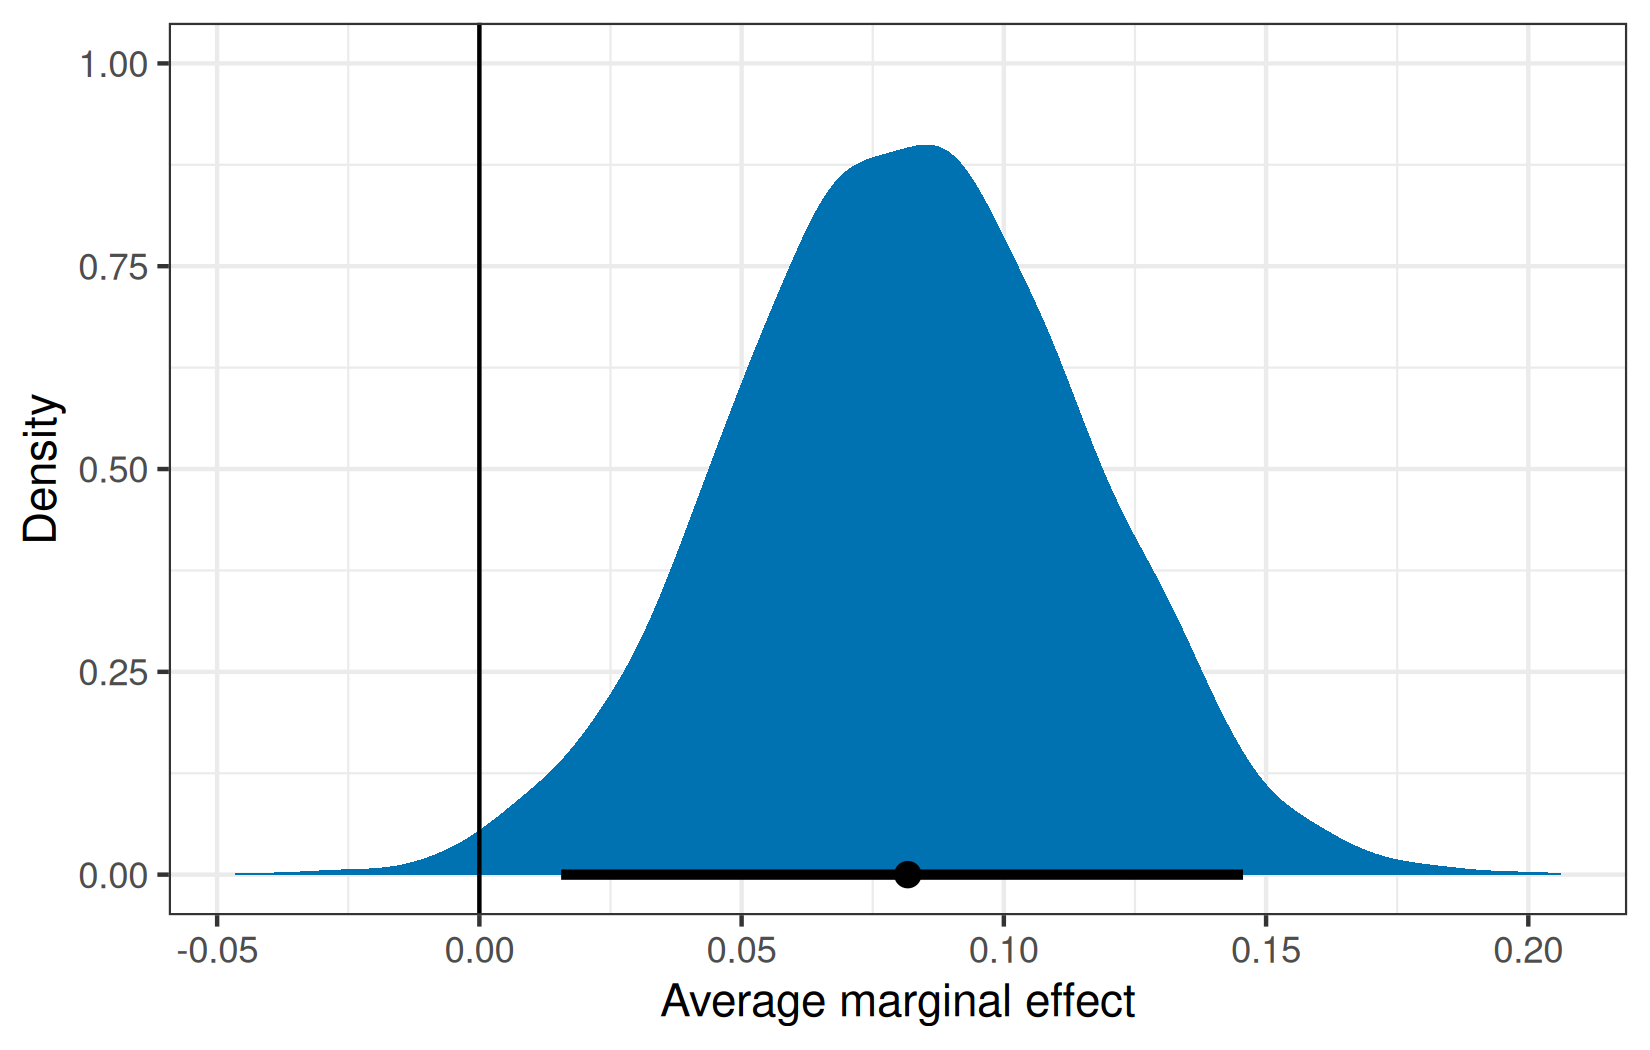
\includegraphics[keepaspectratio]{DoDL_Appendix_files/figure-pdf/fig-bayesmlm-strcomp-1.png}}

}

\subcaption{\label{fig-bayesmlm-strcomp}Strategic Compatibility}

\end{minipage}%
%
\begin{minipage}{0.50\linewidth}

\centering{

\pandocbounded{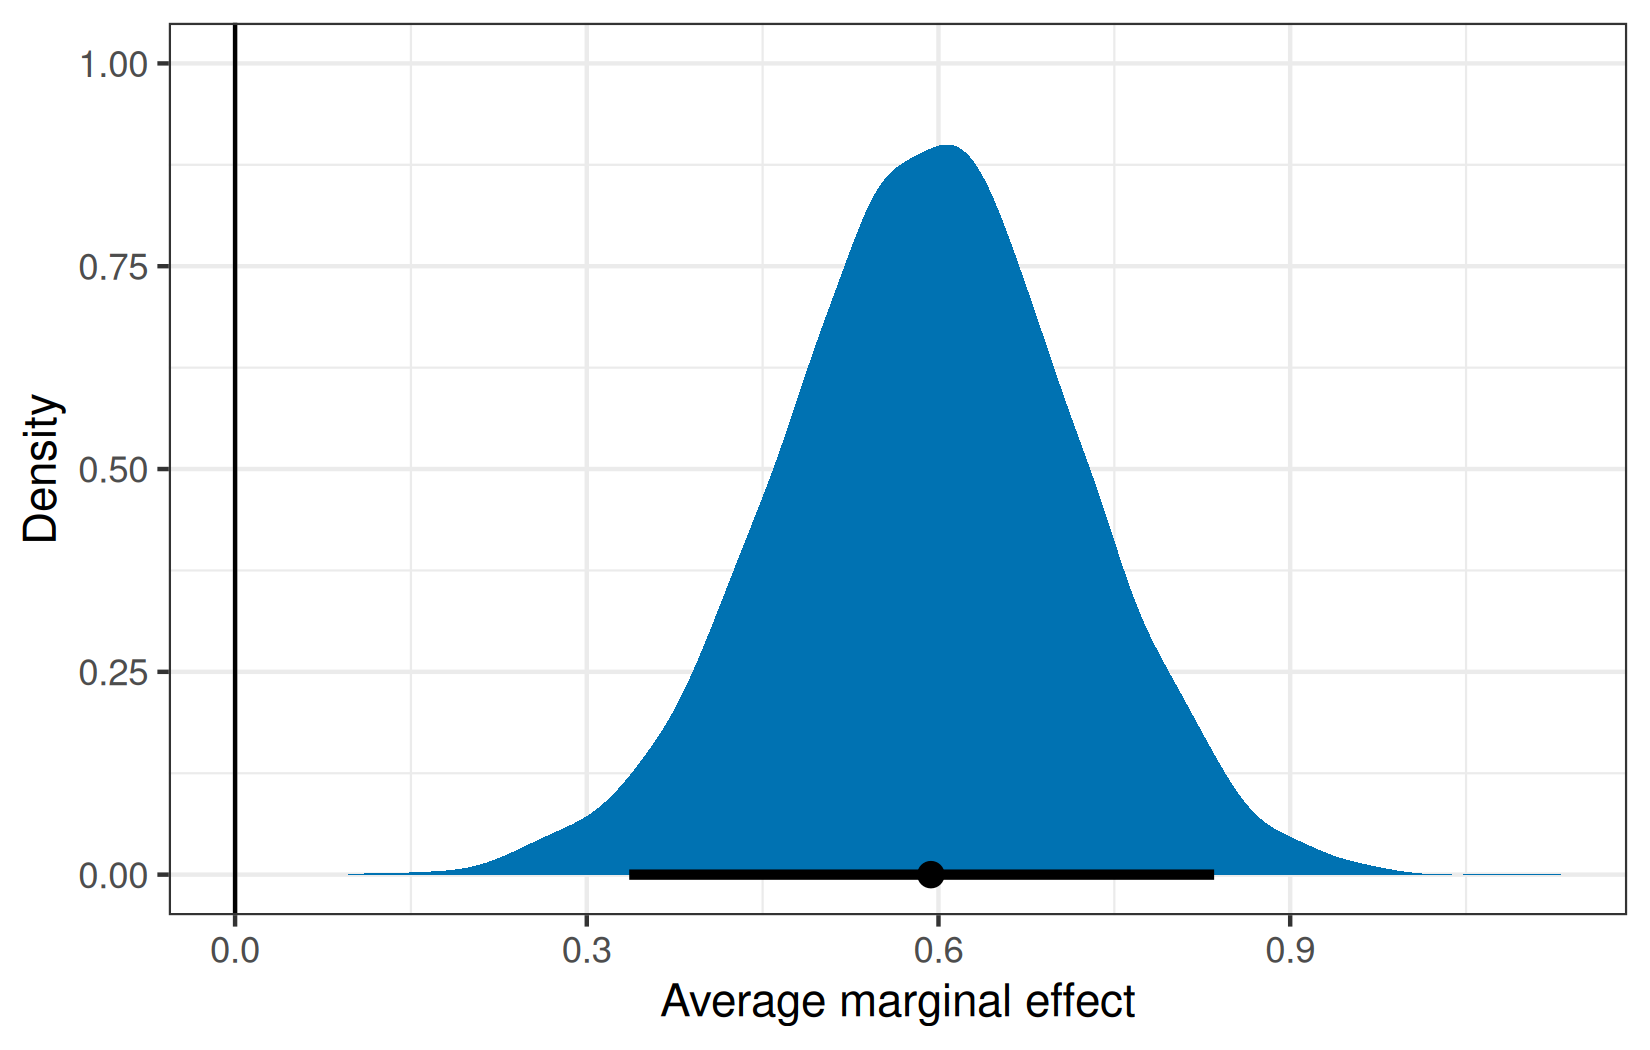
\includegraphics[keepaspectratio]{DoDL_Appendix_files/figure-pdf/fig-bayesmlm-hier-1.png}}

}

\subcaption{\label{fig-bayesmlm-hier}Hierarchy}

\end{minipage}%

\caption{\label{fig-bayesmlm}Average marginal effect on division of
labor of a one standard deviation increase in the independent variables.
Point estimates centered at the median value with 0.95 credible
intervals. Note x-axes are not fixed.}

\end{figure}%

\newpage

\subsection{Double/debiased
Machine-learning}\label{doubledebiased-machine-learning}

Double machine-learning is designed to solve the problem of omitted
variable bias by using the residuals of the control variables and
independent variables to separately predict the dependent variable then
splitting the sample by cross-fitting (Bach et al. 2024).\footnote{Because
  this model can only operate on complete cases, I use the UDS democracy
  score (Marquez 2016; Pemstein, Meserve, and Melton 2017) instead of
  Polity to minimize missing values for the regime type control
  variable.} Table~\ref{tbl-dml} show the results, which are consistent
with the original estimates.

First, the partialling out score function computes the residuals from a
regression of the dependent variable on the control variables then a
regression of the dependent variable on the independent variables. I
then run an OLS of predicting the first stage from the second which
creates valid post-selection inference even in cases of imperfect model
selection by creating a ``second chance'' for omitted variables
(Belloni, Chernozhukov, and Hansen 2014).

This is performed on samples generated using 5-fold re-sampling with one
repeated sample split. The models are cross-fit, meaning I first split
the sample into an auxiliary and a main and estimate the model on the
auxiliary sample then perform the partialling out estimation by OLS on
the main sample. I then reverse the two samples and take the average of
the results, which prevents overfitting (Chernozhukov et al. 2018).

\begin{table}

\caption{\label{tbl-dml}Double/debiased machine learning model.}

\centering{

\centering
\begin{talltblr}[         %% tabularray outer open
entry=none,label=none,
note{}={* p \num{< 0.05}, ** p \num{< 0.01}, *** p \num{< 0.001}},
]                     %% tabularray outer close
{                     %% tabularray inner open
colspec={Q[]Q[]},
column{1}={halign=l,},
column{2}={halign=c,},
hline{6}={1,2}{solid, 0.05em, black},
}                     %% tabularray inner close
\toprule
& (1) \\ \midrule %% TinyTableHeader
Strategic compatibility & \num{0.076}*   \\
& (\num{0.036})  \\
Hierarchy               & \num{0.614}*** \\
& (\num{0.103})  \\
score                   & partialling out \\
n.folds                 & 5               \\
cross.fitting           & TRUE            \\
\bottomrule
\end{talltblr}

}

\end{table}%

\newpage

\section*{Works Cited}\label{works-cited}
\addcontentsline{toc}{section}{Works Cited}

\phantomsection\label{refs}
\begin{CSLReferences}{1}{0}
\bibitem[\citeproctext]{ref-alley_allianceparticipationtreaty_2021}
Alley, Joshua. 2021. {``Alliance {Participation}, {Treaty Depth}, and
{Military Spending}.''} \emph{International Studies Quarterly} 65 (4):
929--43. \url{https://doi.org/10.1093/isq/sqab077}.

\bibitem[\citeproctext]{ref-bach_doublemlobjectorientedimplementation_2024}
Bach, Philipp, Malte S. Kurz, Victor Chernozhukov, Martin Spindler, and
Sven Klaassen. 2024. {``{DoubleML}: {An} Object-Oriented Implementation
of Double Machine Learning in {R}.''} \emph{Journal of Statistical
Software} 108 (3): 1--56. \url{https://doi.org/10/gt3cht}.

\bibitem[\citeproctext]{ref-bailey_estimatingdynamicstate_2017}
Bailey, Michael A., Anton Strezhnev, and Erik Voeten. 2017.
{``Estimating {Dynamic State Preferences} from {United Nations Voting
Data}.''} \emph{Journal of Conflict Resolution} 61 (2): 430--56.
\url{https://doi.org/10.1177/0022002715595700}.

\bibitem[\citeproctext]{ref-bak_allianceproximityeffectiveness_2018}
Bak, Daehee. 2018. {``Alliance {Proximity} and {Effectiveness} of
{Extended Deterrence}.''} \emph{International Interactions} 44 (1):
107--31. \url{https://doi.org/10.1080/03050629.2017.1320995}.

\bibitem[\citeproctext]{ref-bearce_alliancesinternalinformation_2006}
Bearce, David H., Kristen M. Flanagan, and Katharine M. Floros. 2006.
{``Alliances, {Internal Information}, and {Military Conflict Among
Member-States}.''} \emph{International Organization} 60 (3): 595--625.
\url{https://doi.org/10.1017/S0020818306060188}.

\bibitem[\citeproctext]{ref-belloni_inferencetreatmenteffects_2014}
Belloni, Alexandre, Victor Chernozhukov, and Christian Hansen. 2014.
{``Inference on {Treatment Effects} After {Selection} Among
{High-Dimensional Controls}.''} \emph{The Review of Economic Studies} 81
(2): 608--50. \url{https://doi.org/10/f53wkb}.

\bibitem[\citeproctext]{ref-bennett_exploringoperationalizationspolitical_2006}
Bennett, D. Scott. 2006. {``Exploring {Operationalizations} of
{Political Relevance}.''} \emph{Conflict Management and Peace Science}
23 (3): 245--61. \url{https://doi.org/10.1080/07388940600837748}.

\bibitem[\citeproctext]{ref-bennett_durationinterstatewars_1996}
Bennett, D. Scott, and Allan C. Stam. 1996. {``The {Duration} of
{Interstate Wars}, 1816--1985.''} \emph{American Political Science
Review} 90 (2): 239--57. \url{https://doi.org/10/b6zbbd}.

\bibitem[\citeproctext]{ref-benson_assessingvariationformal_2016}
Benson, Brett V., and Joshua D. Clinton. 2016. {``Assessing the
{Variation} of {Formal Military Alliances}.''} \emph{Journal of Conflict
Resolution} 60 (5): 866--98.
\url{https://doi.org/10.1177/0022002714560348}.

\bibitem[\citeproctext]{ref-benson_relevancepoliticallyrelevant_2005}
Benson, Michelle A. 2005. {``The {Relevance} of {Politically Relevant
Dyads} in the {Study} of {Interdependence} and {Dyadic Disputes}.''}
\emph{Conflict Management and Peace Science} 22 (2): 113--33.
\url{https://doi.org/10.1080/07388940590948556}.

\bibitem[\citeproctext]{ref-braumoeller_politicalirrelevancedemocracy_2011}
Braumoeller, Bear F., and Austin Carson. 2011. {``Political
{Irrelevance}, {Democracy}, and the {Limits} of {Militarized
Conflict}.''} \emph{Journal of Conflict Resolution} 55 (2): 292--320.
\url{https://doi.org/10.1177/0022002710393918}.

\bibitem[\citeproctext]{ref-burkner_brmspackagebayesian_2017}
Bürkner, Paul-Christian. 2017. {``Brms: {An R Package} for {Bayesian
Multilevel Models Using Stan}.''} \emph{Journal of Statistical Software}
80 (1): 1--28. \url{https://doi.org/10/gddxwp}.

\bibitem[\citeproctext]{ref-chernozhukov_doubledebiasedmachine_2018}
Chernozhukov, Victor, Denis Chetverikov, Mert Demirer, Esther Duflo,
Christian Hansen, Whitney Newey, and James Robins. 2018.
{``Double/Debiased Machine Learning for Treatment and Structural
Parameters.''} \emph{The Econometrics Journal} 21 (1): 1--68.
\url{https://doi.org/10/gc2snx}.

\bibitem[\citeproctext]{ref-chiba_carefulcommitmentsdemocratic_2015}
Chiba, Daina, Jesse C. Johnson, and Brett Ashley Leeds. 2015. {``Careful
{Commitments}: {Democratic States} and {Alliance Design}.''} \emph{The
Journal of Politics} 77 (4): 968--82.
\url{https://doi.org/10.1086/682074}.

\bibitem[\citeproctext]{ref-cohen_coefficientagreementnominal_1960}
Cohen, Jacob. 1960. {``A {Coefficient} of {Agreement} for {Nominal
Scales}.''} \emph{Educational and Psychological Measurement} 20 (1):
37--46. \url{https://doi.org/10/dghsrr}.

\bibitem[\citeproctext]{ref-diehl_peacedataconcept_2021}
Diehl, Paul F., Gary Goertz, and Yahve Gallegos. 2021. {``Peace Data:
{Concept}, Measurement, Patterns, and Research Agenda.''} \emph{Conflict
Management and Peace Science} 38 (5): 605--24.
\url{https://doi.org/10.1177/0738894219870288}.

\bibitem[\citeproctext]{ref-fordham_allalliancesare_2016}
Fordham, Benjamin O., and Paul Poast. 2016. {``All {Alliances Are
Multilateral}: {Rethinking Alliance Formation}.''} \emph{Journal of
Conflict Resolution} 60 (5): 840--65.
\url{https://doi.org/10.1177/0022002714553108}.

\bibitem[\citeproctext]{ref-gibler_priorcommitmentscompatible_2004}
Gibler, Douglas M., and Toby J. Rider. 2004. {``Prior {Commitments}:
{Compatible Interests} Versus {Capabilities} in {Alliance Behavior}.''}
\emph{International Interactions} 30 (4): 309--29.
\url{https://doi.org/10.1080/03050620490883985}.

\bibitem[\citeproctext]{ref-hage_choicecircumstanceadjusting_2011}
Häge, Frank M. 2011. {``Choice or {Circumstance}? {Adjusting Measures}
of {Foreign Policy Similarity} for {Chance Agreement}.''}
\emph{Political Analysis} 19 (3): 287--305.
\url{https://www.jstor.org/stable/23011439}.

\bibitem[\citeproctext]{ref-hage_consensusdecisionssimilarity_2016}
Häge, Frank M., and Simon Hug. 2016. {``Consensus {Decisions} and
{Similarity Measures} in {International Organizations}.''}
\emph{International Interactions} 42 (3): 503--29.
\url{https://doi.org/10/gtv3zr}.

\bibitem[\citeproctext]{ref-leeds_allianceinstitutionalizationalliance_2005}
Leeds, Brett Ashley, and Sezi Anac. 2005. {``Alliance
{Institutionalization} and {Alliance Performance}.''}
\emph{International Interactions} 31 (3): 183--202.
\url{https://doi.org/10.1080/03050620500294135}.

\bibitem[\citeproctext]{ref-leeds_terminatingallianceswhy_2007}
Leeds, Brett Ashley, and Burcu Savun. 2007. {``Terminating {Alliances}:
{Why Do States Abrogate Agreements}?''} \emph{The Journal of Politics}
69 (4): 1118--32.
\url{https://doi.org/10.1111/j.1468-2508.2007.00612.x}.

\bibitem[\citeproctext]{ref-maoz_domesticsourcesglobal_1996}
Maoz, Zeev. 1996. \emph{Domestic {Sources} of {Global Change}}. Ann
Arbor, MI: University of Michigan Press.
\url{https://doi.org/10.3998/mpub.14663}.

\bibitem[\citeproctext]{ref-marquez_quickmethodextending_2016}
Marquez, Xavier. 2016. {``A {Quick Method} for {Extending} the {Unified
Democracy Scores}.''} \{\{SSRN Scholarly Paper\}\}. Rochester, NY.
\url{https://doi.org/10.2139/ssrn.2753830}.

\bibitem[\citeproctext]{ref-oneal_classicalliberalswere_1997}
Oneal, John R., and Bruce M. Russett. 1997. {``The {Classical Liberals
Were Right}: {Democracy}, {Interdependence}, and {Conflict},
1950--1985.''} \emph{International Studies Quarterly} 41 (2): 267--93.
\url{https://doi.org/10/cnd4m3}.

\bibitem[\citeproctext]{ref-pemstein_democraticcompromiselatent_2017}
Pemstein, Daniel, Stephen A. Meserve, and James Melton. 2017.
{``Democratic {Compromise}: {A Latent Variable Analysis} of {Ten
Measures} of {Regime Type}.''} \emph{Political Analysis} 18 (4):
426--49. \url{https://doi.org/10/bq365m}.

\bibitem[\citeproctext]{ref-poast_arguingalliancesart_2019}
Poast, Paul. 2019. \emph{Arguing about {Alliances}: {The Art} of
{Agreement} in {Military-Pact Negotiations}}. Ithaca: Cornell University
Press.

\bibitem[\citeproctext]{ref-reiter_democracywarinitiation_1998}
Reiter, Dan, and Allan C. Stam. 1998. {``Democracy, {War Initiation},
and {Victory}.''} \emph{American Political Science Review} 92 (2):
377--89. \url{https://doi.org/10.2307/2585670}.

\bibitem[\citeproctext]{ref-shor_bayesianmultilevelmodeling_2007}
Shor, Boris, Joseph Bafumi, Luke Keele, and David Park. 2007. {``A
{Bayesian Multilevel Modeling Approach} to {Time-Series Cross-Sectional
Data}.''} \emph{Political Analysis} 15 (2): 165--81.
\url{https://doi.org/10/bq4db5}.

\bibitem[\citeproctext]{ref-stam_winlosedraw_1996}
Stam, Allan C. 1996. \emph{Win, {Lose}, {Or Draw}: {Domestic Politics}
and the {Crucible} of {War}}. University of Michigan Press.

\bibitem[\citeproctext]{ref-thompson_identifyingrivalsrivalries_2001}
Thompson, William R. 2001. {``Identifying {Rivals} and {Rivalries} in
{World Politics}.''} \emph{International Studies Quarterly} 45 (4):
557--86. \url{https://www.jstor.org/stable/3096060}.

\bibitem[\citeproctext]{ref-thompson_analyzingstrategicrivalries_2021}
Thompson, William R., Kentaro Sakuwa, and Prashant Hosur Suhas. 2021.
\emph{Analyzing {Strategic Rivalries} in {World Politics}: {Types} of
{Rivalry}, {Regional Variation}, and {Escalation}/{De-escalation}}.
Springer Nature.

\bibitem[\citeproctext]{ref-weitsman_intimateenemiespolitics_1997}
Weitsman, Patricia A. 1997. {``Intimate Enemies: {The} Politics of
Peacetime Alliances.''} \emph{Security Studies} 7 (1): 156--93.
\url{https://doi.org/10.1080/09636419708429337}.

\end{CSLReferences}




\end{document}
